\documentclass[10pt,english]{beamer}
%\documentclass[english,handout]{beamer} % For handouts
\usetheme[progressbar=frametitle,block=fill]{metropolis} %numbering=none

%%% USEFUL PACKAGES
%\usepackage{showframe} % For debugging positioning
\usepackage{etex} % If too many packages
% Encoding and language
\usepackage[utf8]{inputenc}
\usepackage{babel}
\usepackage{amsmath, amssymb}
\usepackage{natbib}
%\usepackage{booktabs}
%\usepackage{algorithmic}
\usepackage{algorithm}
\usepackage{caption}
%\usepackage{animate} % Animations
\usepackage{bm} % Bold math
\usepackage{bbm}
%\usepackage{url}
%\usepackage{pifont}
%\usepackage{ulem} % Used for strikeouts \sout
%\usepackage{stackengine}
%\usepackage{enumitem}
%\setlist[description]{leftmargin=\parindent,labelindent=\parindent}
%\usepackage{colortbl} % Used for colored rows in tables


%%% GRAPHICS
\usepackage{graphicx}
\graphicspath{{./figs/}}


%%% COLORS
\setbeamercolor{background canvas}{bg=white}
\def\BlankFrame{
	\bgroup
	%\pdfpageheight 29.7cm
	\setbeamercolor{background canvas}{bg=}
	\begin{frame}[plain]
	\end{frame}
	%\makeatletter
	%\pdfpageheight \beamer@paperheight
	%\makeatother
	\egroup}

\usepackage{xcolor}
\definecolor{DarkGreen}{HTML}{00B200}
\definecolor{LightBlue}{HTML}{0090D9}
\definecolor{gold}{rgb}{.812,.710,.231}
% Text markup
%\setbeamercolor{alerted text}{fg=red}
\newcommand{\blue}[1]{\textcolor{blue}{#1}}
\newcommand{\red}[1]{\textcolor{red}{#1}}
\newcommand{\grey}[1]{\textcolor{gray}{#1}}
\newcommand{\orange}[1]{\textcolor{mLightBrown}{#1}}
\newcommand\myheading[1]{\textbf{#1}}
\newcommand\myemph[1]{\underline{\emph{#1}}}
\newcommand\textexample[1]{\textit{\textbf{#1}}}

%%% SPACING
\newcommand\vws[1][1]{\vspace{#1\baselineskip}} % vertical white space
%\newcommand\strt[1][1.5ex]{\rule[-.05\baselineskip]{0pt}{#1}} % strut
\newcommand\strt[2]{\rule[-#1ex]{0pt}{#2ex}} % strut
\newcommand\Hrule{\vspace{1ex} \hrule \vspace{1ex}} % Horisontal rule with some space after

%%% MISC
\newcommand\articleref[4]{\noindent\begin{minipage}[t]{0.04\textwidth}
		\vspace{0pt} 
		\pgfuseimage{beamericonarticle}
	\end{minipage}%
	\begin{minipage}[t]{0.96\textwidth}
		\vspace{0pt}
		#1. \textbf{#2.} \textit{#3}, #4.
	\end{minipage}}

%%% METROPOLIS THEME SPECIFIC
\makeatletter
\setlength{\metropolis@progressonsectionpage@linewidth}{1pt}
\makeatother
%\setbeamercolor{progress bar}{fg=red,bg=red!50}


%%% TEXTPOS
\usepackage[absolute,overlay]{textpos} % option showboxes is useful in draft mode
\setlength{\TPHorizModule}{\paperwidth}
\setlength{\TPVertModule}{\paperheight}
\textblockorigin{0pt}{10mm} % start everything at top-left, below gray 


%%% TIKZ/PGFPLOTS
\usepackage{tikz}
\usetikzlibrary{arrows,positioning,calc,shapes.geometric}
%\usetikzlibrary{arrows,calc,shapes.geometric,decorations.pathmorphing,backgrounds,positioning,fit,petri,decorations.pathreplacing}
%\usepackage{pgfplots}
%\pgfplotsset{compat = 1.3}


%%% BLOCKS AND BOXES
% Changing colors of blocks
%\setbeamercolor{block title alerted}{bg=UURed,fg=palette primary.fg}
%\setbeamercolor{block body alerted}{bg=UURed!15}
\setbeamercolor{block title alerted}{bg=mLightBrown,fg=palette primary.fg}
\setbeamercolor{block body alerted}{bg=mLightBrown!15}
%\setbeamercolor{block title example}{bg=UUGreen,fg=palette primary.fg}
%\setbeamercolor{block body example}{bg=UUGreen!10}
% \mybox is a rectangular box
\usepackage{boxedminipage}
\setlength\fboxrule{2pt}
\setlength\fboxsep{2\fboxsep}
\newcommand\mybox[3][\textwidth]{
  {\color{#2}
    \begin{boxedminipage}{#1}
      {\color{palette primary.bg} #3}
    \end{boxedminipage}}%
}   
\usepackage{tcolorbox}
\tcbset{arc=1mm,grow to left by=3mm,grow to right by=3mm,left=2mm}
%\newenvironment{redbox}{%
%	\begin{tcolorbox}[colback=UURed!15,colframe=UURed]}{%
%	\end{tcolorbox}}
%\newenvironment{greenbox}{%
%	\begin{tcolorbox}[colback=UUGreen!15,colframe=UUGreen]}{%
%	\end{tcolorbox}}
\newenvironment{redbox}{%
	\begin{tcolorbox}[colback=red!15,colframe=red]}{%
	\end{tcolorbox}}
\newenvironment{greenbox}{%
	\begin{tcolorbox}[colback=DarkGreen!15,colframe=DarkGreen]}{%
	\end{tcolorbox}}
\newenvironment{graybox}{%
	\begin{tcolorbox}[colback=mDarkTeal!5,colframe=mDarkTeal]}{%
	\end{tcolorbox}}
\newenvironment{orangebox}{%
\begin{tcolorbox}[colback=mLightBrown!15,colframe=mLightBrown]}{%
	\end{tcolorbox}}
\newenvironment{bwbox}{%
	\begin{tcolorbox}[colback=white,colframe=black]}{%
\end{tcolorbox}}
\newenvironment{bluebox}{%
	\begin{tcolorbox}[colback=LightBlue!15,colframe=LightBlue]}{%
\end{tcolorbox}}


%%%%%%%%% NEW MACROS

\newcommand\imp[1]{\alert{\textbf{#1}}}
\newcommand\bfit[1]{\textbf{\textit{#1}}}
\newcommand\good{\color{DarkGreen}{$\blacktriangle$}} % used in lists
\newcommand\bad{\color{red}{$\blacktriangledown$}} % used in lists


\RequirePackage{amsmath, amssymb}
\RequirePackage{bbm}
%\RequirePackage{newtxmath}


% Convenience macro for referring to data source
\newcommand\sourceurl[2]{\small \grey{Data from \href{#1}{#2}}}

% Abbreviations
\RequirePackage{xspace}
\newcommand\pdf{pdf\xspace}
\newcommand\ifft{iff\xspace}
\newcommand\ex{\textbf{ex)}\xspace}

% General time series notation
\newcommand\T{n}  % Length of time series
\newcommand\rtheta{{\red{\theta}}}  % Parameter (color coded)
\newcommand\rthetah{{\red{\widehat\theta}}}  % Estimate (color coded)

% Neural netowkrs
\newcommand\h{\mathbf{h}} % Hidden state variable
\newcommand\zz{\mathbf{z}} % Generic input (vector)

% For OLS/AR
\newcommand\noise{\varepsilon}  % This is the noise in AR, but should it be the same as measurement noise in SSM?
\newcommand\noisevar{\sigma^2_\noise}
\newcommand\noisevarhat{\widehat\sigma^2_\noise}
\newcommand\X{\Phi}
\newcommand\y{\mathbf{y}}
\newcommand\bphi{\bm\phi}

% State space models
\newcommand\z{\alpha}  % State vector, general SSM
\newcommand{\obsnoise}{\varepsilon}
\newcommand{\statenoise}{\eta}
\newcommand{\varobs}{\sigma^2_{\varepsilon}}
\newcommand{\varstate}{\sigma^2_{\eta}}
% For structural time series
\newcommand{\trendnoise}{\zeta}
\newcommand{\seasnoise}{\omega}
\newcommand{\vartrend}{\sigma^2_{\trendnoise}}
\newcommand{\varseas}{\sigma^2_{\seasnoise}}

%
\newcommand\FF{T}
\newcommand\GG{R}
\newcommand\HH{Z}
\newcommand{\covobs}{\sigma_\epsilon^2}
\newcommand{\covstate}{Q}
\newcommand\initmean{a_1}
\newcommand\initcov{P_1}
% Kalman filter
\newcommand{\zpart}[2]{\z_{#1}^{#2}}
\newcommand{\wgt}[2]{\omega_{#1}^{#2}}
\newcommand{\wgtsum}[1]{\Omega_{#1}}
\newcommand\zhat[2]{\hat\z_{#1|#2}}
\newcommand\Phat[2]{P_{#1|#2}}
\newcommand\zpred[1]{\zhat{#1}{#1-1}}
\newcommand\Ppred[1]{\Phat{#1}{#1-1}}
\newcommand\zfilt[1]{\zhat{#1}{#1}}
\newcommand\Pfilt[1]{\Phat{#1}{#1}}
\newcommand\ypred[1]{\hat y_{#1|#1-1}}
\newcommand\Spred[1]{F_{#1|#1-1}}
\newcommand\Spredinv[1]{\Spred{#1}^{-1}}
\newcommand\epshat[2]{\hat{\obsnoise}_{#1|#2}}
\newcommand\etahat[2]{\hat{\statenoise}_{#1|#2}}

\newcommand{\statefun}{T}
\newcommand{\obsfun}{Z}
\newcommand{\estfun}{h}

\newcommand{\qd}{q} %State density
\newcommand{\md}{g} %Measure density

\newcommand{\rmd}{\mathrm{d}}

% SMC
\newcommand{\Np}{N}           % Number of particles
\newcommand{\Mp}{M}           % Number of particles in backward simulation



%\RequirePackage{color}
%\newcommand{\flnote}[1]{{\color{red}\textbf{[#1]}}} % Used for notes in text - color red
%\newcommand\Hrule{\vspace{1ex} \hrule \vspace{1ex}} % Horisontal rule with some space after; This is moved to beamer preamble

%%%%%%%%%%%%%%%%%%%%%%%%%%%%%%%%%%%%%%%%%%%%%%%%%%%%%%%%%%%%%%%%%%%%%%%%%%%%%%%%
%                            COMMANDS IN TEXT                                  %
%%%%%%%%%%%%%%%%%%%%%%%%%%%%%%%%%%%%%%%%%%%%%%%%%%%%%%%%%%%%%%%%%%%%%%%%%%%%%%%%
\newcommand\numtext[2]{#1\textsuperscript{#2}}
\newcommand\thsnd[1]{\ensuremath{#1\thinspace000}}
\newcommand{\peqref}[1]{\eqref{#1} on page~\pageref{#1}} % Page referencing for equations: "(1) on page 1"

%%%%%%%%%%%%%%%%%%%%%%%%%%%%%%%%%%%%%%%%%%%%%%%%%%%%%%%%%%%%%%%%%%%%%%%%%%%%%%%%
%                            SPECIFIC MATH                                     %
%%%%%%%%%%%%%%%%%%%%%%%%%%%%%%%%%%%%%%%%%%%%%%%%%%%%%%%%%%%%%%%%%%%%%%%%%%%%%%%%
% Models etc.
%\newcommand{\T}{T}            % Number of samples in data record
\newcommand{\parspace}{\Theta}                                   % Parameter space
\newcommand{\parameter}{\theta}                                  % Parameter
% Spaces
\newcommand{\setX}{\ensuremath{\mathsf{X}}}                      % State-space X
\newcommand{\sigmaX}{\ensuremath{\mathcal{X}}}                   % Sigma algebra on X
\newcommand{\setY}{\ensuremath{\mathsf{Y}}}                      % State-space Y
\newcommand{\sigmaY}{\ensuremath{\mathcal{Y}}}                   % Sigma algebra on Y
\newcommand{\setZ}{\ensuremath{\mathsf{Z}}}                      % State-space Z
\newcommand{\sigmaZ}{\ensuremath{\mathcal{Z}}}                   % Sigma algebra on Z

%%%%%%%%%%%%%%%%%%%%%%%%%%%%%%%%%%%%%%%%%%%%%%%%%%%%%%%%%%%%%%%%%%%%%%%%%%%%%%%%
%                           GENERAL MATH                                       %
%%%%%%%%%%%%%%%%%%%%%%%%%%%%%%%%%%%%%%%%%%%%%%%%%%%%%%%%%%%%%%%%%%%%%%%%%%%%%%%%

% ======== Miscellaneous symbols ========
\newcommand\eqdef{:=}
\newcommand\defeq{=:}
\newcommand\const{\text{const.}}
%\newcommand\eqdef{\stackrel{\text{\scriptsize def}}{=}}

\newcommand\iid{iid}
\newcommand{\iidsim}{\stackrel{\text{\iid}}{\sim}} % iid simulation
\newcommand{\process}[1]{\{#1\}_{t\geq 1}}       % Process (time index t)
\newcommand{\range}[2]{#1, \, \dots, \, #2}      % Range = 1, ..., N
\newcommand{\crange}[2]{\{#1, \, \dots, \, #2\}} % Curly range = {1, ..., N}
\newcommand{\prange}[2]{(#1, \, \dots, \, #2)}   % Parenthesised range = (1, ..., N)
\newcommand{\bwdrange}[2]{#1 : -1 : #2}          % Range = N, ..., 1
\newcommand{\approxpropto}{\stackrel{\sim}\propto}

% Tight dots between \int and \int in a multidimensional integral
\newcommand{\tightcdots}{\hspace*{-0.38em}\cdot\hspace*{-0.3em}\cdot\hspace*{-0.3em}\cdot\hspace*{-0.38em}}

% Arrows - convergence and mappings
% \mapsto                                                     % Mappings, x \mapsto f(x)
\newcommand{\fromto}{\rightarrow}                             % Mapping from set A to set B; f: A \fromto B
\newcommand{\goesto}{\rightarrow}                             % limits used in n \goesto \infty
\newcommand{\goestosmall}{\to}                                % limits used in \lim_{n \goestosmall \infty}
\newcommand{\convP}{\stackrel{\probab}\longrightarrow}        % Convergence in probability
\newcommand{\convD}{\stackrel{\textrm{D}}\longrightarrow}     % Convergence in distribution

% ======== Standard spaces  ========
\newcommand{\naturals}{\ensuremath{\mathbb{N}}}               % Natural numbers
\newcommand{\reals}{\ensuremath{\mathbb{R}}}                  % Real numbers
\newcommand{\nonnegatives}{\reals_{\smaller +}}               % Nonnegative numbers
\newcommand{\positives}{\reals_{\smaller ++}}                 % Positive numbers
\newcommand{\nonnegativedefinites}[1]{S_{\smaller +}(#1)}     % Nonnegative #1 x #1 matrices
\newcommand{\positivedefinites}[1]{S_{++}(#1)}                % Positive #1 x #1 matrices

% ======== Matrices ========
\newcommand{\eye}[1]{I_{#1}}                     % Identity matrix
\newcommand{\+}{\mathsf{T}}                      % Transpose
\newcommand{\kronecker}{\raisebox{1pt}{\ensuremath{\otimes}}} % Kronecker product
\DeclareMathOperator*\diag{diag}
\DeclareMathOperator*\trace{tr}

% ======== Operators, calculus etc. ========
\newcommand{\Ordo}{O}                            % Big ordo
\newcommand{\supnorm}[1]{\|#1\|_\infty}          % Supremum norm
\newcommand\osc{\text{osc}}                      % Oscillator norm
\newcommand{\grad}{\nabla}                       % Gradient
\newcommand{\complementof}[1]{\ensuremath{#1^\mathsf{c}}} % Set complement
\renewcommand\vec{\text{vec}}
\DeclareMathOperator*\supp{supp}                          % Support
\DeclareMathOperator*\card{card}                          % Set cardinality
\DeclareMathOperator*\rank{rank}                          % Rank
\DeclareMathOperator*\sign{sign}                          % Signum function
\DeclareMathOperator*\argmax{arg\,max}
\DeclareMathOperator*\argmin{arg\,min}

% ======== Probability ========
\newcommand{\Prb}{\ensuremath{\mathbb{P}}}                       % Probability
\newcommand{\E}{\ensuremath{\mathbb{E}}}                         % Expectation
\newcommand{\var}{\ensuremath{\mathrm{Var}}}                     % Variance
\newcommand{\cov}{\ensuremath{\mathrm{Cov}}}                     % Covariance
\newcommand{\cor}{\ensuremath{\mathrm{Corr}}}                     % Correlation
\newcommand{\I}{\ensuremath{\mathbbm{1}}}						 % Indicator function

%\newcommand{\abscont}{\ensuremath{\ll}}          % Absolute continuity
\renewcommand\mid{\,\vert\,} % I don't really like that \mid produces rubber lengths. Sometimes, we get very large white spaces p(x    |   y), and it can produce line breaks after "p(x |" . Is the non-rubber definition here better?
\newcommand\Mid{\,\middle\vert\,} % Stretchable |, to use with \left \right - N.B. This produces a longer | in general. Does that look better than a standard \mid?


% Distributions
\newcommand{\N}{\ensuremath{\mathcal{N}}}        % Normal
\newcommand{\uni}{\ensuremath{\mathcal{U}}}      % Uniform
\newcommand\MN{\mathcal{MN}}                     % Matrix normal
\newcommand\IW{\mathcal{IW}}                     % Inverse-Wishart
\newcommand\GP{\mathcal{GP}}                     % Gaussian process
\DeclareMathOperator*\Mult{Mult}                 % Multinomial
\DeclareMathOperator*\cat{Cat}                   % Categorical
\DeclareMathOperator*\Discrete{Discrete}         % Categorical/alternative name
\DeclareMathOperator*\bin{Bin}                   % Binomial
\DeclareMathOperator*\gam{Gam}                   % Gamma
\DeclareMathOperator*\St{St}                     % Student's t
\DeclareMathOperator*\po{Po}                   % Binomial

%\usepackage{extendedalt}
%\usepackage{animate} % Animations
%\usepackage{../lindsten}
%\usepackage{movie15}
\usepackage{tikz}
\usepackage{listofitems} % for \readlist to create arrays

\title{732G12 Data Mining}
\subtitle{Föreläsning 8}
\date{}
\author{Johan Alenlöv \\ IDA, Linköping University, Sweden}
\titlegraphic{\hfill
\includegraphics[height=1.2cm]{../LiU_primary_black.pdf}}
%\institute{Joint work with\dots}


%% MY DEF %%
\newcommand{\itm}[1]{\mathrm{Item}_{#1}}
\newcommand{\pausa}{\pause}
%\renewcommand{\pausa}{}
\tikzstyle{mynode}=[thick,draw=blue,fill=blue!20,circle,minimum size=22]


\newenvironment{nscenter}
 {\parskip=0pt\par\nopagebreak\centering}
 {\par\noindent\ignorespacesafterend}

\begin{document}

\maketitle

\begin{frame}{Dagens föreläsning}

    \begin{itemize}
        \item K-medoid klustring
        \item Densitetsbaserade metoder
        \item Faktorer som påverkar klusteranalys
        \item Utvärdera klusteranalys
    \end{itemize}
    
\end{frame}

\begin{frame}{Information Kandidatuppsats}
    
    Kommer (troligtvis) vara ett informationsmöte om kandidatuppsatsen på torsdag nästa vecka. 

\end{frame}

\begin{frame}{K-medoid klustring}

    Använder \imp{medioder} som center/prototyp vid klustring.
    \begin{itemize}
        \item En \imp{mediod} är en representativ observation inom ett dataset/kluster.
        \item Mediod är \imp{inte} samma som centroid, median, geometrisk median etc.
        \item Medioder är \imp{lätta att tolka}
        \begin{itemize}
            \item centroider kan vara punkter som inte liknar någon av observationerna i data.
        \end{itemize}
        \item k-mediods:
        \begin{itemize}
            \item minimerar summan av parvisa avstånd.
            \item kan använda godtyckligt avståndsmått.
            \item mer robust med brus och extremvärden.
        \end{itemize}
        \item k-means: använder oftast euklidiskt avstånd.
        \item k-mediod klustring kallas också Partitioning Around Medoids (PAM)
    \end{itemize}
    
\end{frame}

\begin{frame}{K-medoid klustring}

    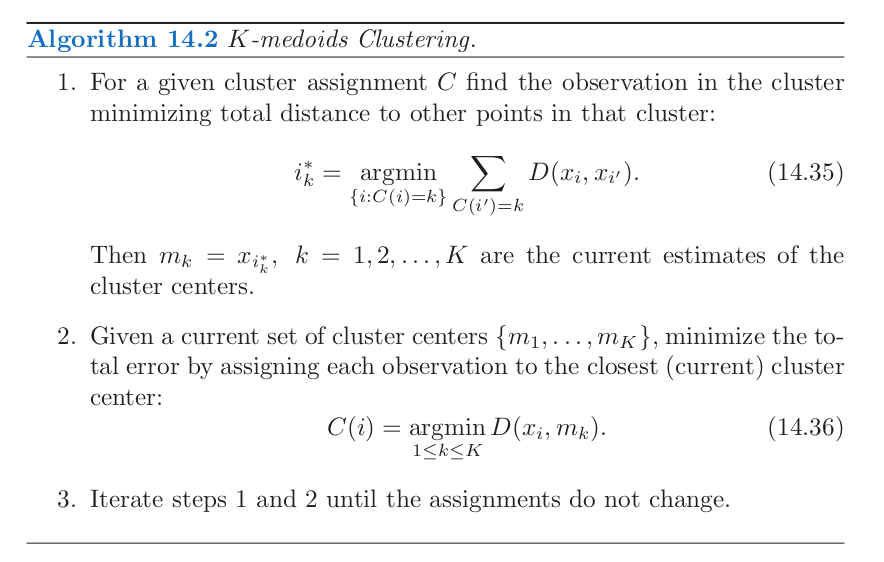
\includegraphics[width = \textwidth]{figs/k-mediod.png}
    
\end{frame}

\begin{frame}{Densitetsbaserade metoder}

    Kluster kan formas baserat på hur densiteten på punkter varierar över variablerna: Täta områden kan defineras som ett kluster.

    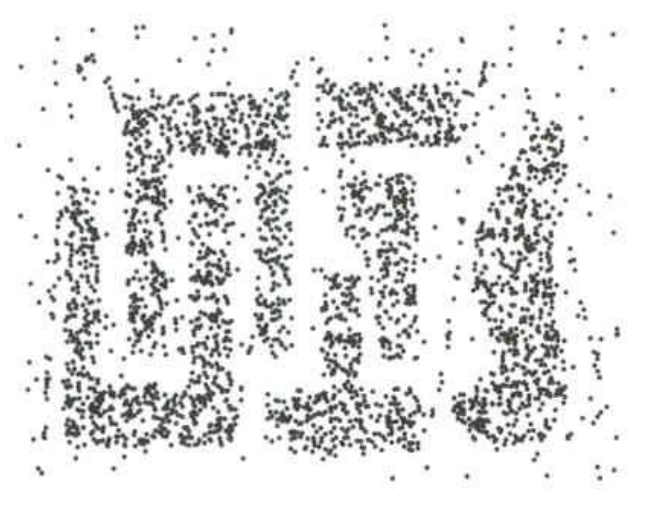
\includegraphics[width = .8\textwidth]{figs/density_cluster2.png}
    
\end{frame}

\begin{frame}{DBSCAN}

    \begin{itemize}
        \item Algoritm för att skapa kluster baserat på punkternas täther.
        \item Använder två begrepp:
        \begin{itemize}
            \item $\operatorname{eps}$, en sökradie där vi letar efter punkter.
            \item $\operatorname{minPts}$, minsta antal punkter.
        \end{itemize}
    \end{itemize}
    
    Från detta kan vi klassa observation i någon av följande:
    \begin{description}
        \item[Kärnpunkt] Punkter med fler än $\operatorname{minPts}$ punkter inom sökradien $\operatorname{eps}$.
        \item[Gränspunkt] Inte en kärnpunkt men hamnar inom sökradien från en kärnpunkt.
        \item[Bruspunkt] Varken kärnpunkt eller gränspunkt.   
    \end{description}

\end{frame}

\begin{frame}{Illustration}
    
    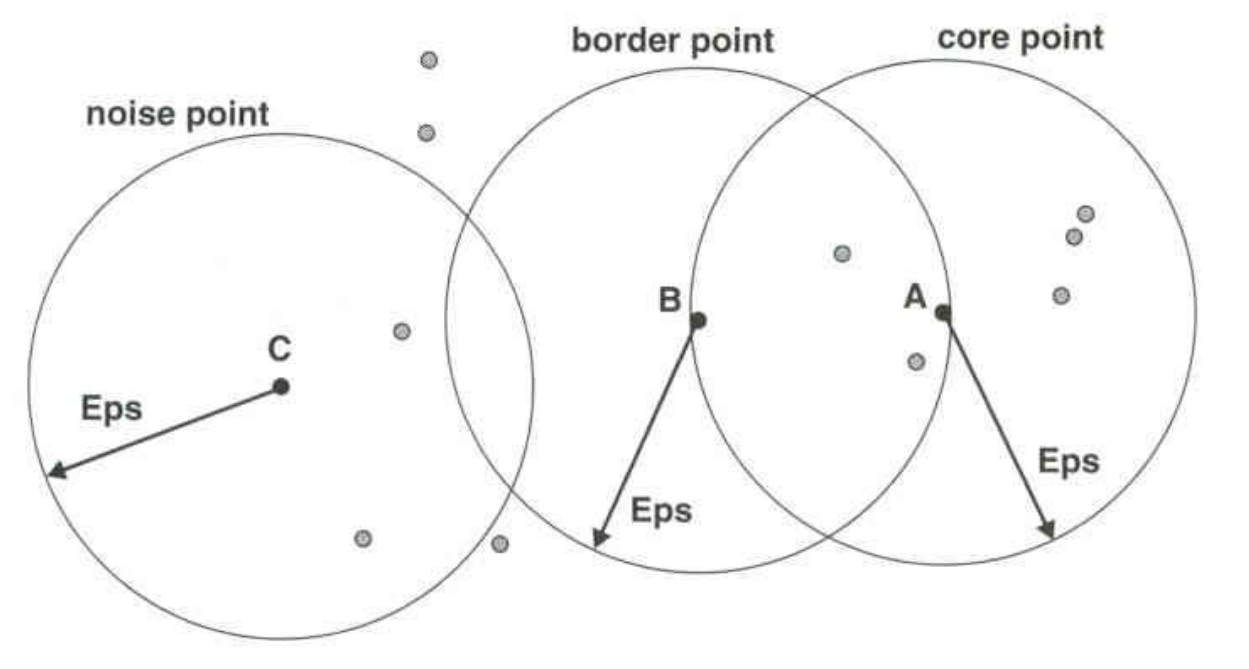
\includegraphics[width=\textwidth]{figs/DBSCAN_obs_class.png}

\end{frame}

\begin{frame}{DBSCAN Algoritmen}

    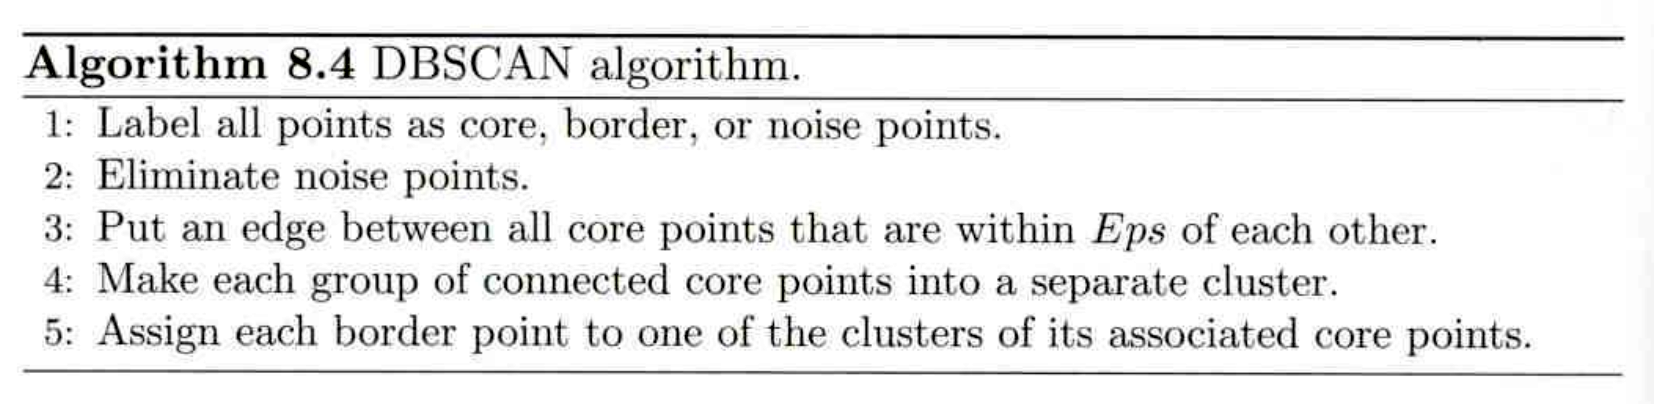
\includegraphics[width=\textwidth]{figs/DBSCAN algoritm.png}
    
\end{frame}

\begin{frame}{Val av $\operatorname{eps}$ och $\operatorname{minPts}$}

    Hyperparametrar som vi måste välja.
    \begin{enumerate}
        \item Definera ett nummer $k$.
        \item Beräkna avståndet mellan varje punkt och dess $k$-närmaste granne och sortera punkterna enligt ökande avstånd.
        \item Definera $\operatorname{eps}$ som värdet där skarp förändring märks (armbågsmetoden).
        \item $\operatorname{minPts} = k$.
    \end{enumerate}
    $k$-värdet vi valt i steg 1 påverkar \imp{inte} $\operatorname{eps}$-värdet mycket om $k$ inte är extremt (för litet eller för stort).
    
\end{frame}

\begin{frame}{DBSCAN - Exempel}

    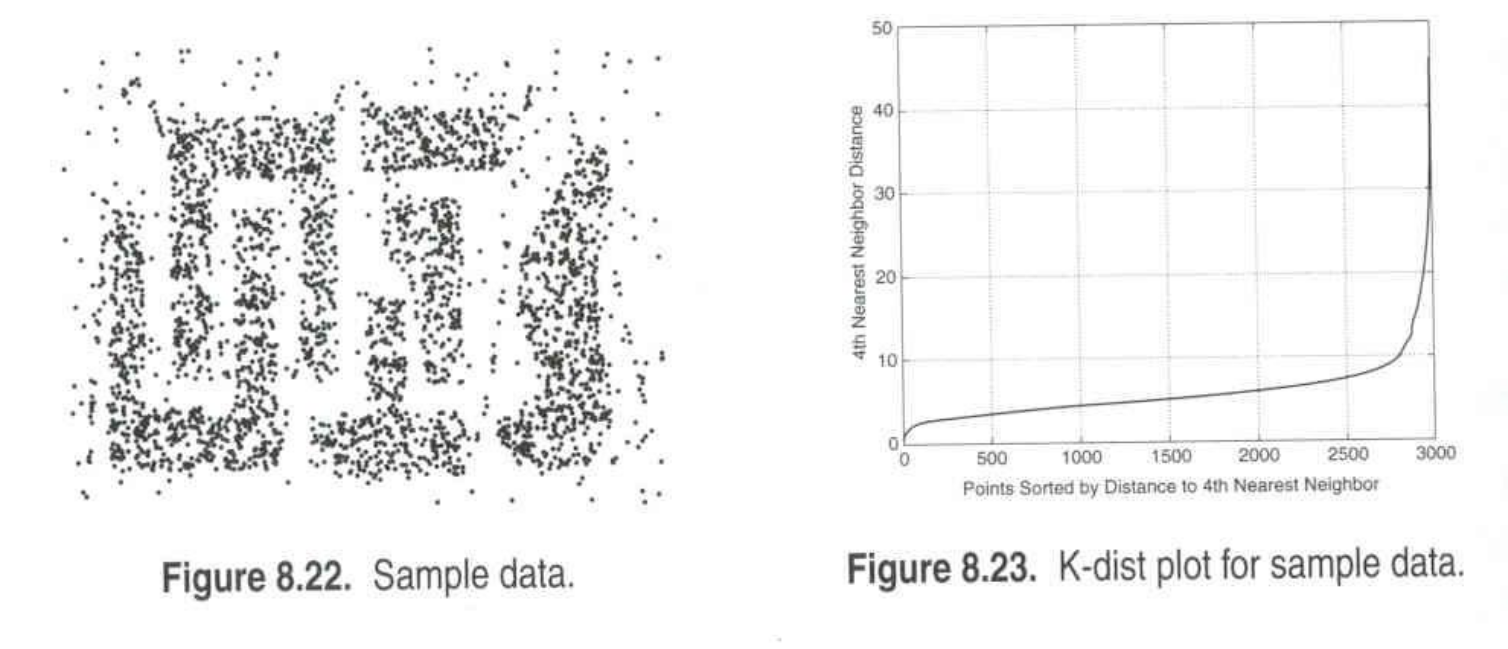
\includegraphics[width=\textwidth]{figs/density_cluster.png}
    
\end{frame}

\begin{frame}{DBSCAN - Exempel}
    
    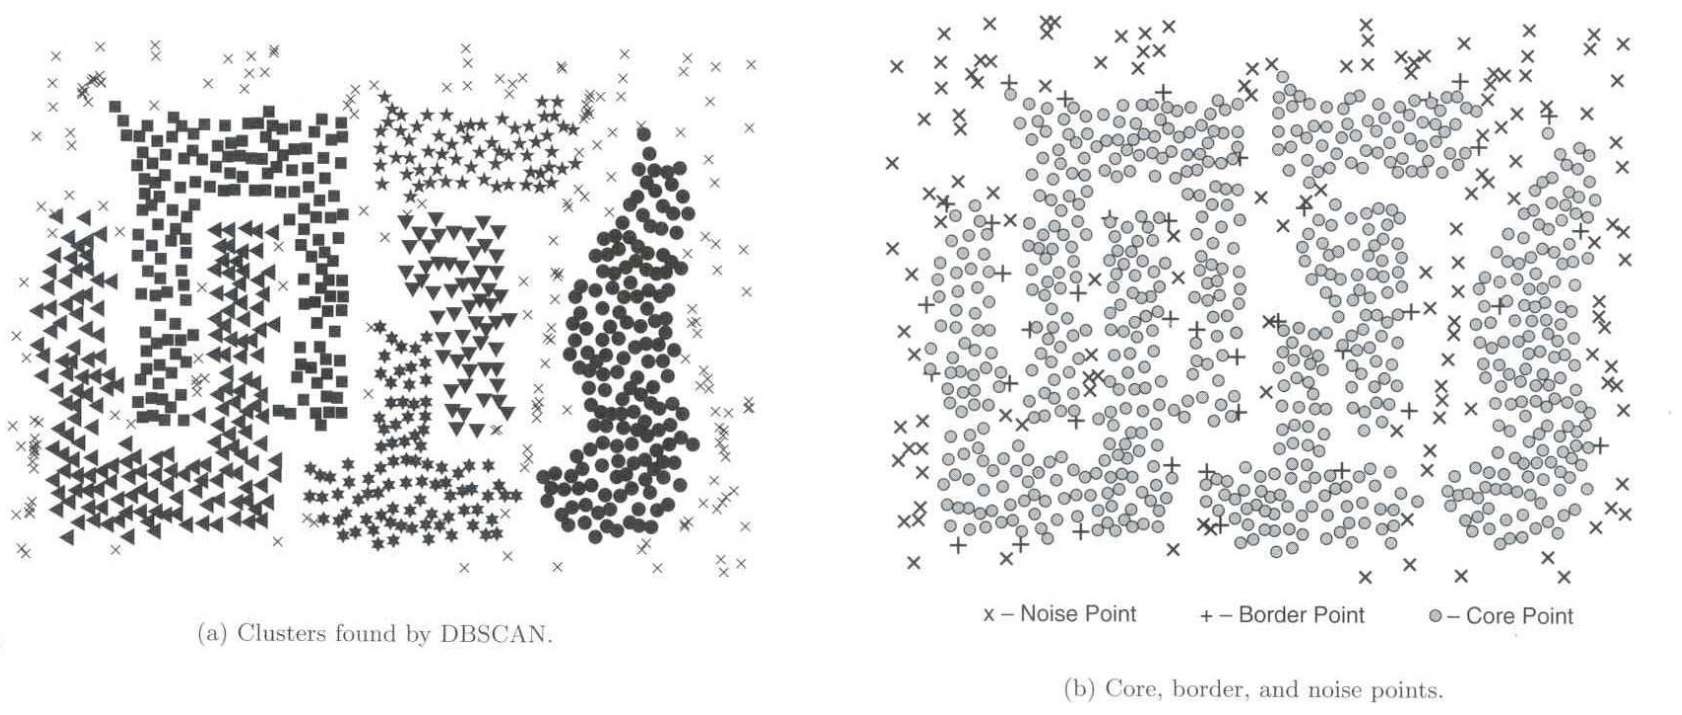
\includegraphics[width=\textwidth]{figs/DBSCAN_cluster_example.png}

\end{frame}

\begin{frame}{DBSCAN - För och nackdelar}

    \begin{itemize}
        \item Brusbeständig.
        \item Behandlar kluster av olika former och storlekar.
        \item Problem med kluster som har betydligt varierande tätheter.
        \begin{itemize}
            \item Svårt att välja ett bra $\operatorname{eps}$.
        \end{itemize}
        \item Problem i stora dimensioner.
    \end{itemize}
    
\end{frame}

\begin{frame}{K-means och DBSCAN}

    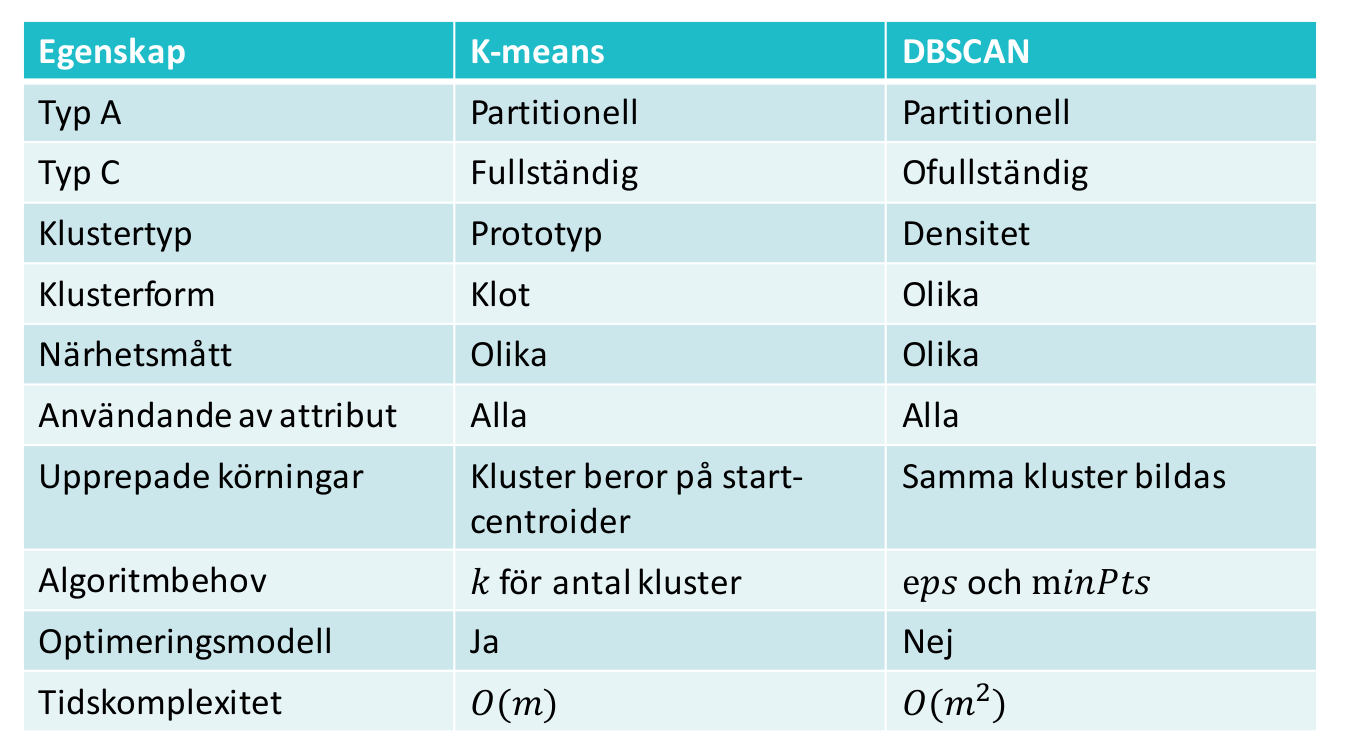
\includegraphics[width=\textwidth]{figs/compre_k-mean_DBACAN.png}
    
\end{frame}

\begin{frame}{Faktorer som påverkar klusteranalys}
    \begin{itemize}
        \item Dimensionalitet (problem för täthetsbaserade metoder).
        \item Datamängdens storlek (stora datamängder är svåra att skala upp).
        \item Brus och extremvärden.
        \item Skalan på data: numerisk, kategorisk.
        \begin{itemize}
            \item problem att välja närhetsmått för datamängder med blandade attribut.
        \end{itemize}
        \item Standardisering av variabler.
    \end{itemize}
\end{frame}

\begin{frame}{Egenskaper}
    
\begin{itemize}
    \item Fördelningar - Olika metoder passar bättre på vissa fördelningar.
    \item Form - Godtyckliga former är svårare att klustra.
    \item Storlek - K-means, problem med olika storlekar.
    \item Tåthet - Olika täthet problem för K-means, DBSCAN.
    \item Dålgit separerade kluster - Vissa metoder slår ihop överlappande kluster.
\end{itemize}

\begin{redbox}
Ingen klustermetod passar för alla dataset!
\end{redbox}

\end{frame}

\begin{frame}{Utvärdera klusteranalys}

    \begin{itemize}
        \item Cluster tendency: Finns det kluster i data? Eller har observationerna bara slumpmässiga värden?
        \item Avgöra rätt antal kluster.
        \item Interna mått på hur bra klusteranalysen är.
        \item Externa mått på hur bra klusteranalysen är, om vi har tillgång till sanna klasser/grupper.
        \item Jämföra olika metoder för klusteranalys på samma dataset.
        \item Kontext och problembeskrivning, avgör om vi har en bra klustring.
    \end{itemize}
    
\end{frame}

\begin{frame}{Cohesion och Separation}
    Interna mått.
    \begin{description}
        \item[Cohesion:] Hur tight eller sammanhållet ett kluster är med sig själv.
        \item[Separation:] Hur väl separerat ett kluster är från övriga kluster.
    \end{description}
    
    När vi har beräknat mått för ett kluster kan vi väga samman alla dessa mått till ett mått.

\end{frame}

\begin{frame}{Cohesion och Separation}
    
    \begin{align*}
        \operatorname{cohesion}(C_i) &= \sum_{x \in C_i, y \in C_i} \operatorname{proximity}(x,y) \\
        \operatorname{proximity}(C_i, C_j) &= \sum_{x \in C_i, y \in C_j} \operatorname{proximity}(x,y)
    \end{align*}

    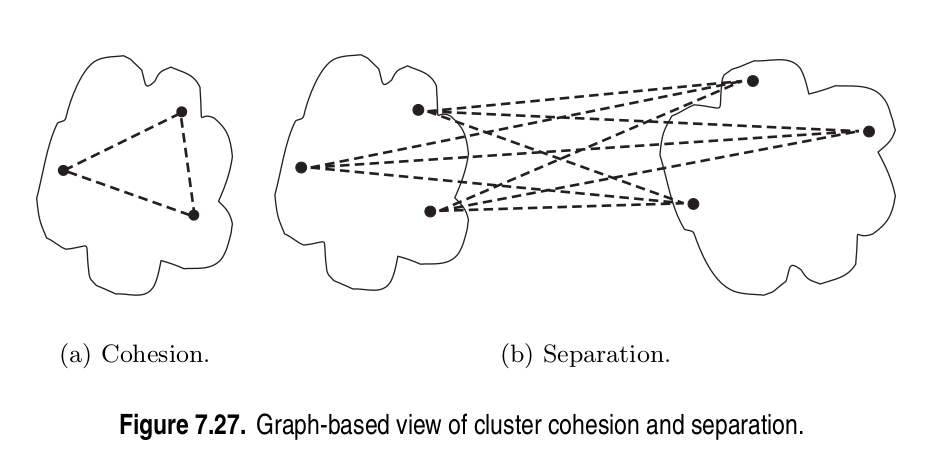
\includegraphics[width=.8\textwidth]{figs/cohesion and separation.1.png}

    $\operatorname{proximity}(x,y)$ kan vara både närhetsmått eller avståndsmått.

\end{frame}

\begin{frame}{The Silhouette Coefficient}
    
    Använder både cohesion och separation för att beräkna ett mått.

    \begin{enumerate}
        \item Beräkna medelavståndet från $\text{observation}_i$ till alla andra observationer i dess kluster, kalla det $a_i$.
        \item Beräkna nu medelavståndet från $\text{observation}_i$ till alla kluster som inte innehåller denna observation.
        \item Hitta det minsta av dessa avstånd kalla det $b_i$.
        \item Silhouette coefficient för $\text{observation}_i$ defineras som,
        \begin{equation*}
            s_i = \frac{b_i - a_i}{\max(a_i, b_i)}
        \end{equation*}
    \end{enumerate}

\end{frame}

\begin{frame}{The Silhouette Coefficient}

    \begin{equation*}
        s_i = \frac{b_i - a_i}{\max(a_i, b_i)}
    \end{equation*}

    \begin{itemize}
        \item $s_i$ kan ta värden mellan $-1$ och $1$.
        \item 1 är bästa möjliga värde.
        \begin{itemize}
            \item Vill ha $a_i < b_i$ och att $a_i$ ska vara nära noll.
        \end{itemize}
        \item Average silhouette coefficient.
        \begin{itemize}
            \item Ta medelvärdet över alla $s_i$
            \item Ger ett mått på hur bra klustringen är.
        \end{itemize}
    \end{itemize}
    
\end{frame}

\begin{frame}{The Silhouette Coefficient - Exempel}

    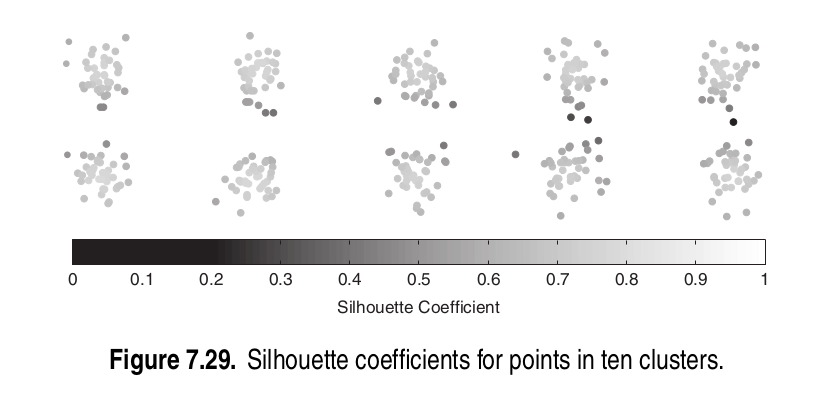
\includegraphics[width=\textwidth]{figs/Silhouette coefficients for points in ten clusters..png}
    
\end{frame}

\begin{frame}{Välja antal kluster}

    \begin{itemize}
        \item K-means: vi kan använda total SSE och average silhouette coefficient.
        \item Plotta dessa mot antal kluster.
        \begin{itemize}
            \item Kolla efter böjar och toppar.
            \item SSE planar ut efter en böj: ta antal kluster vid böjen.
            \item Average silhouette coefficient: Kolla om det finns en eller flera toppar.
        \end{itemize}
    \end{itemize}
    
\end{frame}

\begin{frame}{Välja antal kluster - Exempel}

    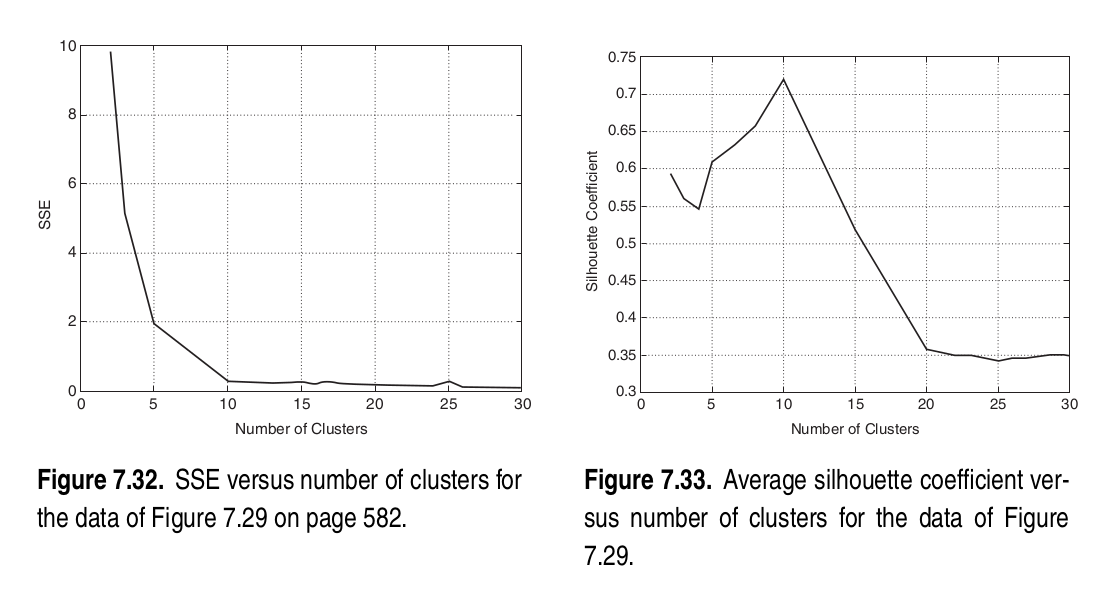
\includegraphics[width=\textwidth]{figs/Determining the Correct Number of Clusters.png}
    
\end{frame}

\begin{frame}{Calinski-Harabasz Index}
    \begin{description}
        \item[Inter-cluster dispersion]
        \begin{equation*}
            \operatorname{BGSS} = \sum_{k=1}^{K} n_k \| C_k - C \|^2.
        \end{equation*}
        \item[Intra-cluster dispersion]
        \begin{equation*}
            \operatorname{WGSS}_k = \sum_{i=1}^{n_k} \| x_{i,k} - C_k \|^2, \qquad \operatorname{WGSS} = \sum_{k=1}^{K} \operatorname{WGSS}_k.
        \end{equation*}
        \item[Calinski-Harabasz Index]
        \begin{equation*}
            \operatorname{CH} = \frac{\operatorname{BGSS}}{\operatorname{WGSS}} \cdot \frac{N - K}{K-1}.
        \end{equation*}
    \end{description}
    Höga värden är bra för CH.

    Davies-Bouldin Index är ett liknande mått. Där ska man ha låga värden.
\end{frame}

\begin{frame}{Välja antal kluster}

    \begin{itemize}
        \item Vi kan beräkna närhetsmatrisen eller avståndsmatrisen för alla datapunkter.
        \begin{itemize}
            \item Matris med alla parvisa närheter/avstånd mellan observationer.
        \end{itemize}
        \item Notera att detta är dyrt!
        \begin{itemize}
            \item Kostar $O(n^2)$
            \item Svårt att plotta med många observationer.
            \item En lösning är att ta ett slumpmässigt urval av data.
        \end{itemize}
        \item Sortera närhetsmatrisen baserat på kluster.
        \begin{itemize}
            \item Först kommer kluster 1, sen kluster 2, osv.
        \end{itemize}
        \item Om vi har väl separerade kluster och valt ett bra antal kluster kommer den sorterade matrisen vara ungefär blockdiagonal.
    \end{itemize}
    
\end{frame}

\begin{frame}{Välja antal kluster - Exempel}

    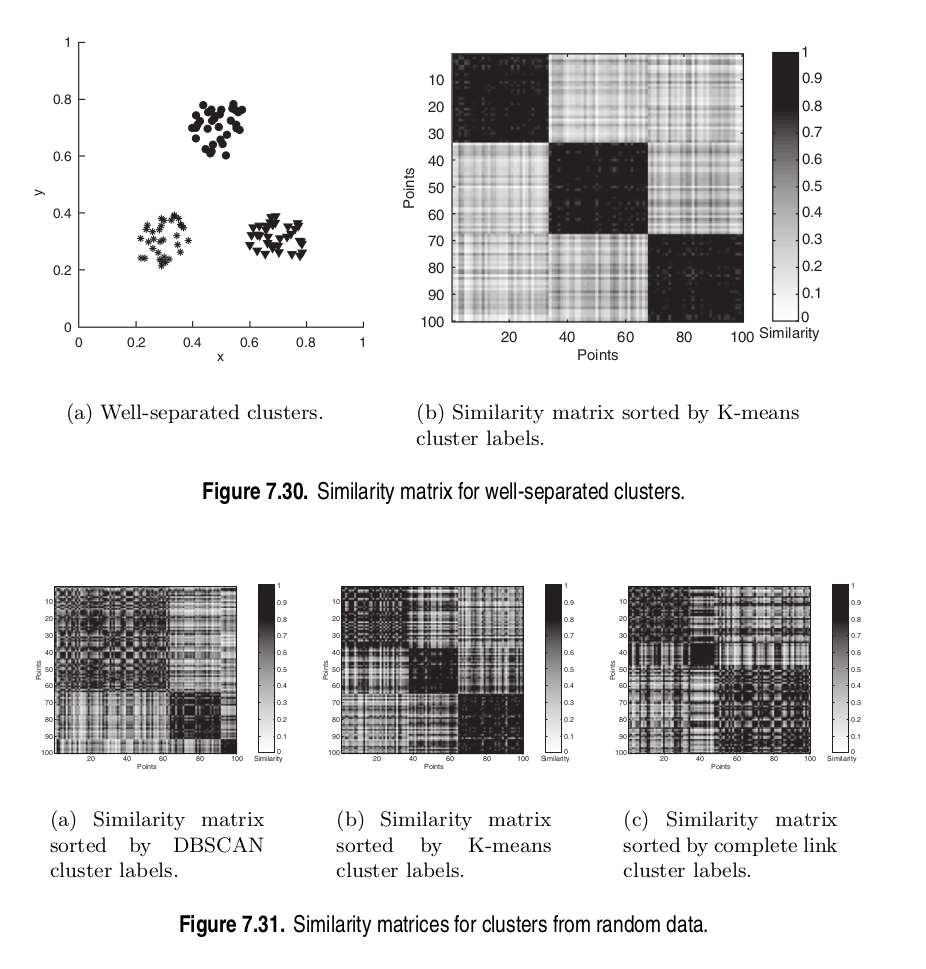
\includegraphics[width=.8\textwidth]{figs/Similarity matrices for clusters.png}
    
\end{frame}

\begin{frame}{Cluster Tendency}

    \begin{itemize}
        \item Har vi slumpmässig data eller finns det något mönster? (kluster)
        \item Sampla två grupper om $p$ datapunkter
        \begin{itemize}
            \item Uniformt fördelade från datarymden.
            \item Från datasetet utan återläggning.
        \end{itemize}
        \item Beräkna avståndet till närmaste granne i datasetet.
        \begin{itemize}
            \item $u_i$ är minsta avståndet från en uniform datapunkt till en observation.
            \item $w_i$ är minsta avståndet från en samplad datapunkt till en icke-samplad datapunkt.
        \end{itemize}
        \item Hopkins statistic:
        \begin{equation*}
            \operatorname{H} 0 \frac{\sum_{i=1}^{p}w_i}{\sum_{i=1}^{p}u_i + \sum_{i=1}^{p}w_i}
        \end{equation*}
        \item Nollhypotesen är att datasetet följer en uniform fördelning. $\operatorname{H}$ kommer då vara $\operatorname{Beta}(p,p)$ fördelat.
        \item Värden nära 1 indikerar att data inte är uniformt fördelat.
        
    \end{itemize}
    
\end{frame}

\begin{frame}{Extern validering}

    \begin{itemize}
        \item Jämför med sanna klasser/kluster.
        \item Vi kan ta resultatet från vår klusteranalys som våra "predikterade värden"
        \item Kan då jämföra med sanna klasserna.
        \begin{itemize}
            \item Vi kan då beräkna förväxlingsmatris och liknande mått.
        \end{itemize}
        \item Notera:
        \begin{itemize}
            \item Vi har inte de "rätta namnen" på våra kluster.
            \item Vi vill ofta att klustren ska vara så rena som möjligt, dvs. domineras av en klass.
        \end{itemize}
    \end{itemize}
    
\end{frame}

\end{document}